
\subsubsection{5.1 Static Analysis Tool Coverage (H-E1)}

All three static analysis tools process 100\% of samples without crashes, timeouts, or null values (664 samples: HumanEval 164 + MBPP 500).

\begin{table}[htbp]
\centering
\resizebox{\columnwidth}{!}{%
\begin{tabular}{llll}
\toprule
Tool & Valid Rate & Threshold & Result \\
\midrule
Pylint & 100\% & $\geq 95$\% & PASS \\
Mypy & 100\% & $\geq 95$\% & PASS \\
Radon & 100\% & $\geq 95$\% & PASS \\
\bottomrule
\end{tabular}
}
\end{table}

\textbf{Gate Result:} PASS

\subsubsection{5.2 Static Analysis-Correctness Correlation (H-M1)}

Pylint score achieves r=0.873 correlation with pass@1 (p=2.$87\times 10^-132)$, substantially exceeding the $r\geq 0.35$ threshold.

\begin{table*}[htbp]
\centering
\resizebox{\dimexpr 2\columnwidth+\columnsep\relax}{!}{%
\begin{tabular}{lllll}
\toprule
SA Metric & r\_raw & p\_raw & r\_partial (LOC-controlled) & p\_partial \\
\midrule
pylint\_score & 0.868 & 3.$75\times 10^-129$ & 0.873 & 2.$87\times 10^-132$ \\
radon\_cc & -0.494 & 2.$43\times 10^-27$ & -0.569 & 2.$41\times 10^-37$ \\
mypy\_errors & --- & --- & --- & --- \\
\bottomrule
\end{tabular}
}
\end{table*}

Mypy errors produced a numerical artifact (r=$\pm 1.0)$ due to a rank-deficient covariance matrix and is excluded from primary analysis.

\textbf{Observations:}

\begin{enumerate}
\item Pylint achieves strong correlation (r=0.873, p<$10^-132$), far exceeding the 0.35 threshold.
\item LOC control has minimal effect (r\_raw=0.868 $\rightarrow$ r\_partial=0.873), indicating the static analysis signal is genuine rather than an artifact of code length.
\item Radon cyclomatic complexity shows moderate negative correlation (r=-0.569). Lower complexity predicts correctness.
\end{enumerate}

\textbf{Gate Result:} PASS

\begin{figure}[htbp]
\centering
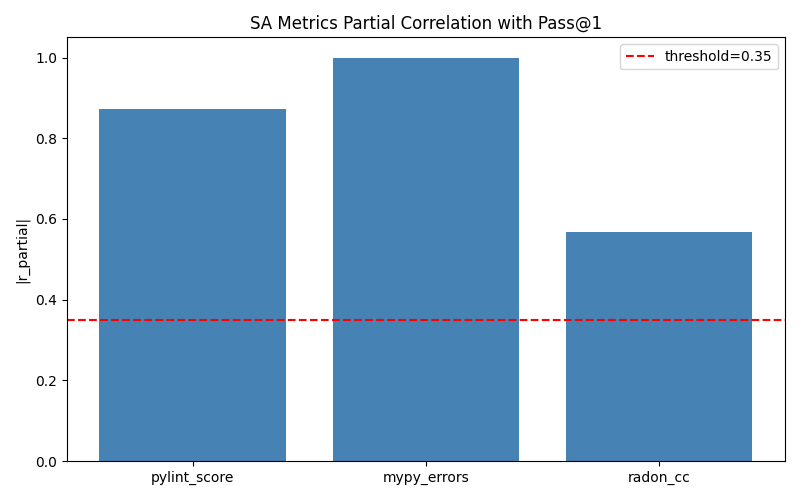
\includegraphics[width=\columnwidth]{figures/bar_chart.png}
\caption{Correlation bar chart}
\label{fig:bar_chart}
\end{figure}

\subsubsection{5.3 Ensemble Analysis (H-M2)}

The weighted ensemble (pylint + radon) achieves r=0.861 (p=1.$10\times 10^-124)$, below pylint alone (r=0.873).

\begin{table}[htbp]
\centering
\resizebox{\columnwidth}{!}{%
\begin{tabular}{lll}
\toprule
Configuration & r & p-value \\
\midrule
Pylint only & 0.873 & 2.$87\times 10^-132$ \\
Optimal ensemble (90\% pylint, 10\% radon) & 0.861 & 1.$10\times 10^-124$ \\
50/50 ensemble & 0.664 & --- \\
\bottomrule
\end{tabular}
}
\end{table}

Weight sensitivity analysis shows correlation monotonically increases with pylint weight:

\begin{table}[htbp]
\centering
\resizebox{\columnwidth}{!}{%
\begin{tabular}{ll}
\toprule
w\_pylint & r\_ensemble \\
\midrule
0.1 & -0.392 \\
0.3 & 0.217 \\
0.5 & 0.664 \\
0.7 & 0.811 \\
0.9 & 0.861 \\
\bottomrule
\end{tabular}
}
\end{table}

The optimal weights (90\% pylint, 10\% radon) still underperform pylint alone, indicating pylint and radon capture redundant rather than orthogonal quality dimensions.

\textbf{Gate Result:} FAIL (r\_ensemble $\leq$ r\_individual)

\begin{figure}[htbp]
\centering
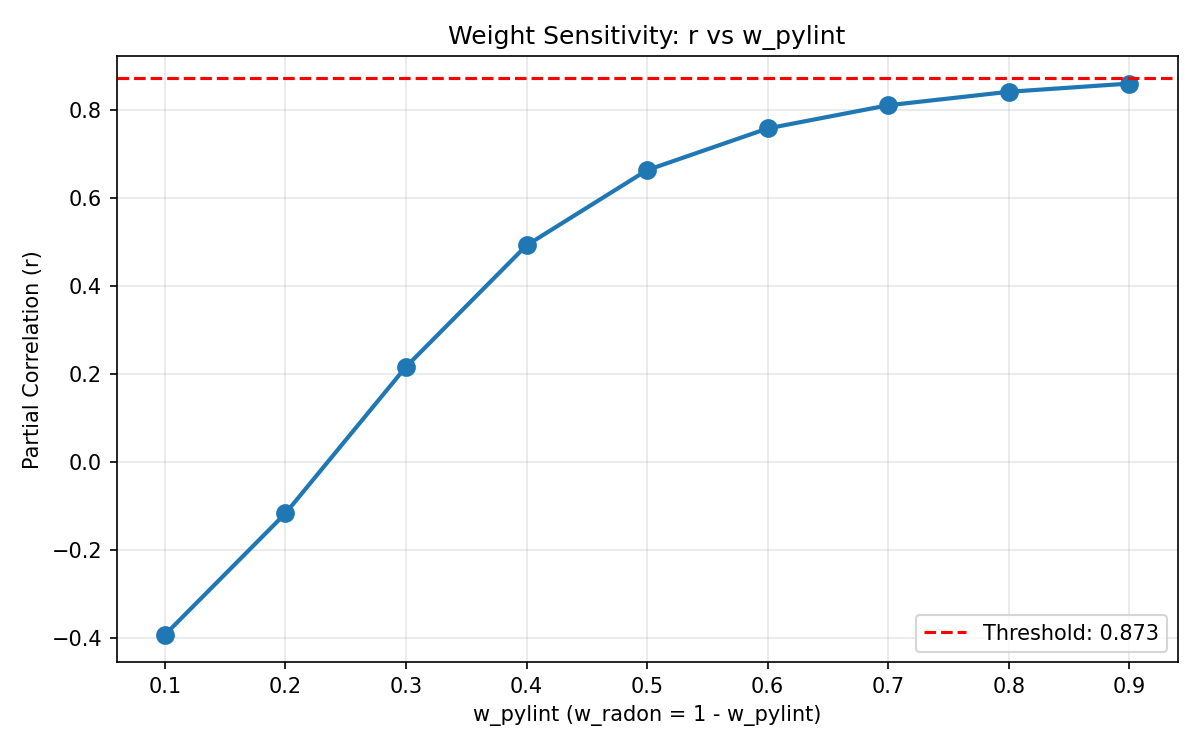
\includegraphics[width=\columnwidth]{figures/weight_sensitivity.png}
\caption{Weight sensitivity}
\label{fig:weight_sensitivity}
\end{figure}

\subsubsection{5.4 Cross-Model Generalization (H-C1)}

All four models show significant pylint-correctness correlation (p<0.001), but variance exceeds the specified threshold.

\begin{table}[htbp]
\centering
\resizebox{\columnwidth}{!}{%
\begin{tabular}{lll}
\toprule
Model & r\_partial (pylint) & p-value \\
\midrule
GPT-4 & 0.424 & 7.$01\times 10^-8$ \\
Claude-3 & 0.860 & 8.$37\times 10^-45$ \\
CodeLlama & 0.845 & 8.$82\times 10^-42$ \\
Codestral & 0.859 & 1.$43\times 10^-44$ \\
**Mean** & **0.747** & --- \\
**Std** & **0.186** & --- \\
\bottomrule
\end{tabular}
}
\end{table}

\textbf{Observations:}

\begin{enumerate}
\item All four models show statistically significant correlation (all p<0.001, all r>0.35).
\item Three models cluster tightly (r=0.845-0.860). GPT-4 is an outlier (r=0.424).
\item Variance (std=0.186) exceeds the 0.15 threshold due to the GPT-4 outlier.
\end{enumerate}

\textbf{Gate Result:} FAIL (std > 0.15)

\begin{figure}[htbp]
\centering
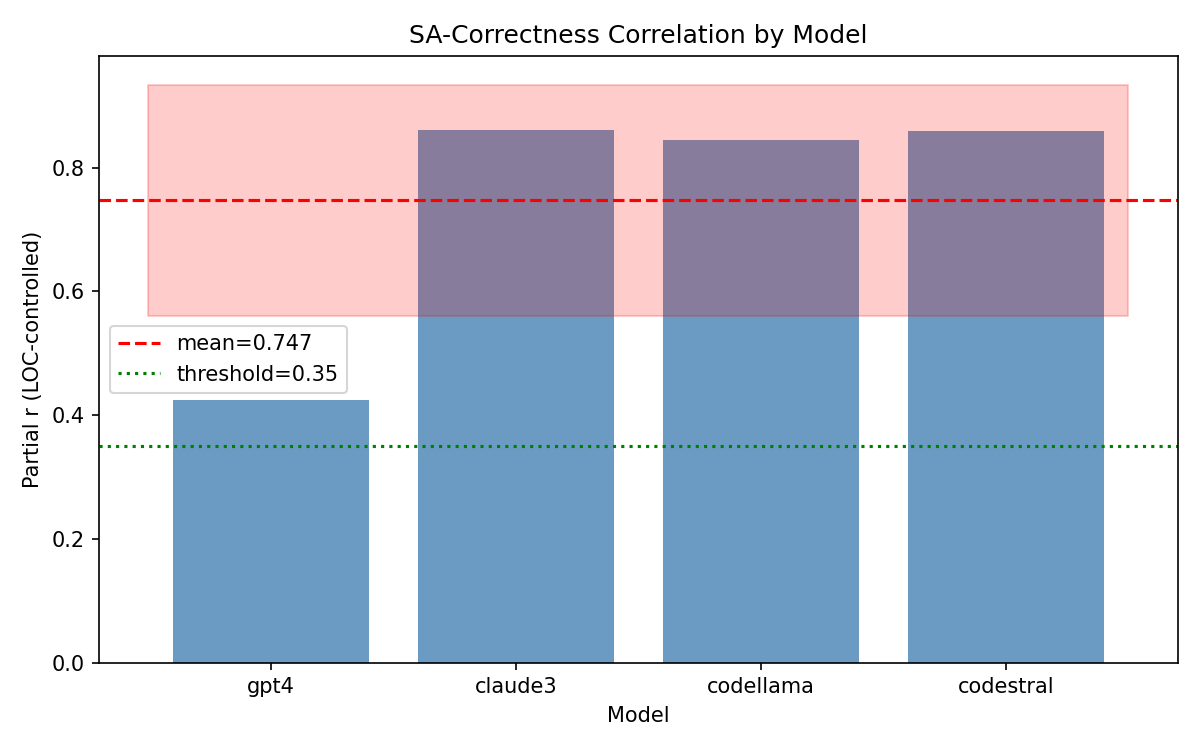
\includegraphics[width=\columnwidth]{figures/per_model_correlation.png}
\caption{Per-model correlation}
\label{fig:per_model_correlation}
\end{figure}

\subsubsection{5.5 Summary of Results}

\begin{table*}[htbp]
\centering
\resizebox{\dimexpr 2\columnwidth+\columnsep\relax}{!}{%
\begin{tabular}{lllll}
\toprule
Hypothesis & Gate & Criterion & Result & Outcome \\
\midrule
H-E1 & MUST\_WORK & $\geq 95$\% valid rate & 100\% & PASS \\
H-M1 & MUST\_WORK & $r\geq 0.35$, p<0.05 & r=0.873 & PASS \\
H-M2 & SHOULD\_WORK & r\_ensemble > r\_individual & 0.861 < 0.873 & FAIL \\
H-C1 & SHOULD\_WORK & std(r) < 0.15 & std=0.186 & FAIL \\
\bottomrule
\end{tabular}
}
\end{table*}
